%!TeX encoding = UTF-8
%!TeX program = xelatex
\documentclass[notheorems, aspectratio=54]{beamer}
% aspectratio: 1610, 149, 54, 43(default), 32

\usepackage{latexsym}
\usepackage{amsmath,amssymb}
\usepackage{mathtools}
\usepackage{color,xcolor}
\usepackage{graphicx}
\usepackage{algorithm}
\usepackage{amsthm}
\usepackage{lmodern} % 解决 font warning
% \usepackage[UTF8]{ctex}
\usepackage{animate} % insert gif
\usepackage{lipsum} % To generate test text 
\usepackage{ulem} % 下划线,波浪线

\usepackage{listings} % display code on slides; don't forget [fragile] option after \begin{frame}

% ----------------------------------------------
% tikx
\usepackage{framed}
\usepackage{tikz}
\usepackage{pgf}
% ----------------------------------------------

% ------------ added by fengyuan----------------
% \usepackage{amsfonts}       % blackboard math symbols
% ----------------------------------------------

\usetikzlibrary{calc,trees,positioning,arrows,chains,shapes.geometric,%
    decorations.pathreplacing,decorations.pathmorphing,shapes,%
    matrix,shapes.symbols}
\pgfmathsetseed{1} % To have predictable results
% Define a background layer, in which the parchment shape is drawn
\pgfdeclarelayer{background}
\pgfsetlayers{background,main}

% define styles for the normal border and the torn border
\tikzset{
  normal border/.style={orange!30!black!10, decorate, 
     decoration={random steps, segment length=2.5cm, amplitude=.7mm}},
  torn border/.style={orange!30!black!5, decorate, 
     decoration={random steps, segment length=.5cm, amplitude=1.7mm}}}

% Macro to draw the shape behind the text, when it fits completly in the
% page
\def\parchmentframe#1{
\tikz{
  \node[inner sep=2em] (A) {#1};  % Draw the text of the node
  \begin{pgfonlayer}{background}  % Draw the shape behind
  \fill[normal border] 
        (A.south east) -- (A.south west) -- 
        (A.north west) -- (A.north east) -- cycle;
  \end{pgfonlayer}}}

% Macro to draw the shape, when the text will continue in next page
\def\parchmentframetop#1{
\tikz{
  \node[inner sep=2em] (A) {#1};    % Draw the text of the node
  \begin{pgfonlayer}{background}    
  \fill[normal border]              % Draw the ``complete shape'' behind
        (A.south east) -- (A.south west) -- 
        (A.north west) -- (A.north east) -- cycle;
  \fill[torn border]                % Add the torn lower border
        ($(A.south east)-(0,.2)$) -- ($(A.south west)-(0,.2)$) -- 
        ($(A.south west)+(0,.2)$) -- ($(A.south east)+(0,.2)$) -- cycle;
  \end{pgfonlayer}}}

% Macro to draw the shape, when the text continues from previous page
\def\parchmentframebottom#1{
\tikz{
  \node[inner sep=2em] (A) {#1};   % Draw the text of the node
  \begin{pgfonlayer}{background}   
  \fill[normal border]             % Draw the ``complete shape'' behind
        (A.south east) -- (A.south west) -- 
        (A.north west) -- (A.north east) -- cycle;
  \fill[torn border]               % Add the torn upper border
        ($(A.north east)-(0,.2)$) -- ($(A.north west)-(0,.2)$) -- 
        ($(A.north west)+(0,.2)$) -- ($(A.north east)+(0,.2)$) -- cycle;
  \end{pgfonlayer}}}

% Macro to draw the shape, when both the text continues from previous page
% and it will continue in next page
\def\parchmentframemiddle#1{
\tikz{
  \node[inner sep=2em] (A) {#1};   % Draw the text of the node
  \begin{pgfonlayer}{background}   
  \fill[normal border]             % Draw the ``complete shape'' behind
        (A.south east) -- (A.south west) -- 
        (A.north west) -- (A.north east) -- cycle;
  \fill[torn border]               % Add the torn lower border
        ($(A.south east)-(0,.2)$) -- ($(A.south west)-(0,.2)$) -- 
        ($(A.south west)+(0,.2)$) -- ($(A.south east)+(0,.2)$) -- cycle;
  \fill[torn border]               % Add the torn upper border
        ($(A.north east)-(0,.2)$) -- ($(A.north west)-(0,.2)$) -- 
        ($(A.north west)+(0,.2)$) -- ($(A.north east)+(0,.2)$) -- cycle;
  \end{pgfonlayer}}}

% Define the environment which puts the frame
% In this case, the environment also accepts an argument with an optional
% title (which defaults to ``Example'', which is typeset in a box overlaid
% on the top border
\newenvironment{parchment}[1][Example]{%
  \def\FrameCommand{\parchmentframe}%
  \def\FirstFrameCommand{\parchmentframetop}%
  \def\LastFrameCommand{\parchmentframebottom}%
  \def\MidFrameCommand{\parchmentframemiddle}%
  \vskip\baselineskip
  \MakeFramed {\FrameRestore}
  \noindent\tikz\node[inner sep=1ex, draw=black!20,fill=white, 
          anchor=west, overlay] at (0em, 2em) {\sffamily#1};\par}%
{\endMakeFramed}

% ----------------------------------------------

\mode<presentation>{
    \usetheme{CambridgeUS}
    % Boadilla CambridgeUS
    % default Antibes Berlin Copenhagen
    % Madrid Montpelier Ilmenau Malmoe
    % Berkeley Singapore Warsaw
    \usecolortheme{beaver}
    % beetle, beaver, orchid, whale, dolphin
    \useoutertheme{infolines}
    % infolines miniframes shadow sidebar smoothbars smoothtree split tree
    \useinnertheme{circles}
    % circles, rectanges, rounded, inmargin
}
% 设置 block 颜色
\setbeamercolor{block title}{bg=red!30,fg=white}

\newcommand{\reditem}[1]{\setbeamercolor{item}{fg=red}\item #1}

% 缩放公式大小
\newcommand*{\Scale}[2][4]{\scalebox{#1}{\ensuremath{#2}}}

% 解决 font warning
\renewcommand\textbullet{\ensuremath{\bullet}}

% ---------------------------------------------------------------------
% flow chart
\tikzset{
    >=stealth',
    punktchain/.style={
        rectangle, 
        rounded corners, 
        % fill=black!10,
        draw=white, very thick,
        text width=6em,
        minimum height=2em, 
        text centered, 
        on chain
    },
    largepunktchain/.style={
        rectangle,
        rounded corners,
        draw=white, very thick,
        text width=10em,
        minimum height=2em,
        on chain
    },
    line/.style={draw, thick, <-},
    element/.style={
        tape,
        top color=white,
        bottom color=blue!50!black!60!,
        minimum width=6em,
        draw=blue!40!black!90, very thick,
        text width=6em, 
        minimum height=2em, 
        text centered, 
        on chain
    },
    every join/.style={->, thick,shorten >=1pt},
    decoration={brace},
    tuborg/.style={decorate},
    tubnode/.style={midway, right=2pt},
    font={\fontsize{10pt}{12}\selectfont},
}
% ---------------------------------------------------------------------

% code setting
\lstset{
    language=C++,
    basicstyle=\ttfamily\footnotesize,
    keywordstyle=\color{red},
    breaklines=true,
    xleftmargin=2em,
    numbers=left,
    numberstyle=\color[RGB]{222,155,81},
    frame=leftline,
    tabsize=4,
    breakatwhitespace=false,
    showspaces=false,               
    showstringspaces=false,
    showtabs=false,
    morekeywords={Str, Num, List},
}

% ---------------------------------------------------------------------

%% preamble
\title[Diffusion Models in Protein Design]{Diffusion Models in Protein Design}
% \subtitle{The subtitle}
\author{Fengyuan Dai}
\institute[Westlake University]{daifengyuan@westlake.edu.cn}

% -------------------------------------------------------------

\begin{document}

%% title frame
\begin{frame}
    \titlepage
\end{frame}

%% normal frame
\section{Denoising Diffusion Probabilistic Models}
\begin{frame}
    \frametitle{Table of Contents}
    \tableofcontents[currentsection]
\end{frame}


\begin{frame}{Denoising Diffusion Probabilistic Models}
  \vspace{-3mm}
  \begin{figure}[!h]
      \centering
      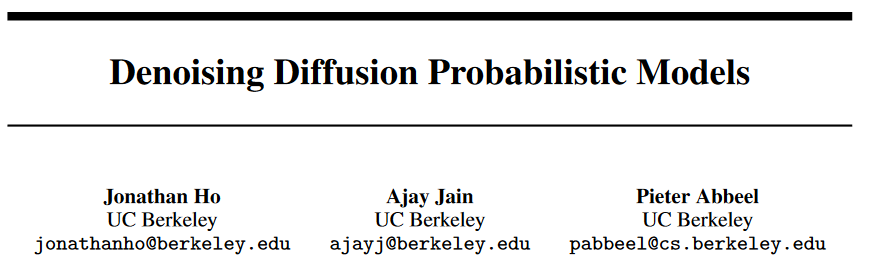
\includegraphics[width=0.9\linewidth]{figures/ddpm.png}
      % 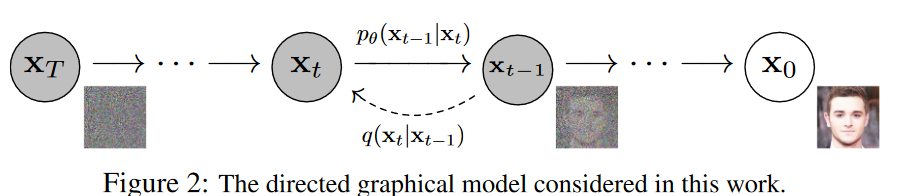
\includegraphics[width=0.8\linewidth]{figures/ddpm_fig2.png}
  \end{figure}
  \begin{itemize}
    \item A diffusion model is a parameterized Markov chain trained using    \\
    variational inference to produce samples matching the data after finite time.
  \end{itemize}
  \vspace{-3mm}
  \begin{figure}[!h]
    \centering
    % 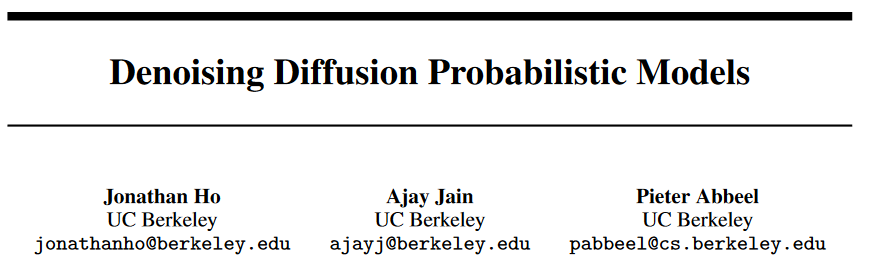
\includegraphics[width=1\linewidth]{figures/ddpm.png}
    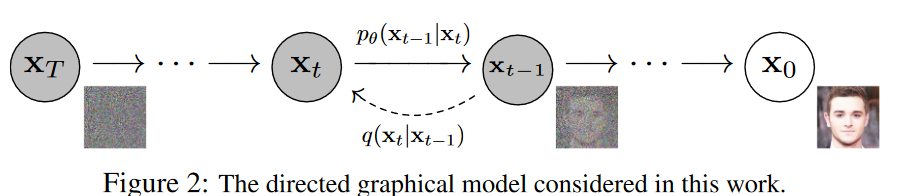
\includegraphics[width=0.8\linewidth]{figures/ddpm_fig2.png}
\end{figure}
\end{frame}

\begin{frame}{Denoising Diffusion Probabilistic Models}
  \begin{figure}[!h]
      \centering
      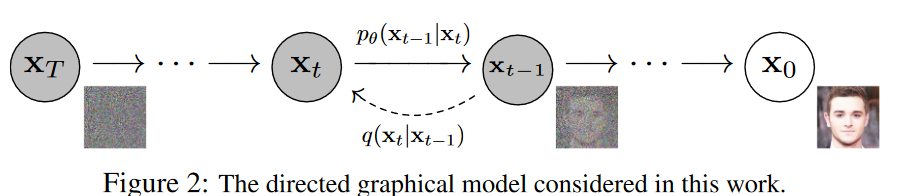
\includegraphics[width=0.8\linewidth]{figures/ddpm_fig2.png}
  \end{figure}
  \begin{itemize}
    \item Forword Process:
    \begin{figure}[!h]
      \centering
      
\includegraphics[width=1.0\linewidth]{figures/ddpm_formulation2.png}
    \end{figure}
    \item Reverse Process:
    \begin{figure}[!h]
      \centering
      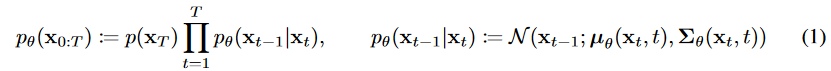
\includegraphics[width=1.0\linewidth]{figures/ddpm_formulation1.png}
    \end{figure}
  \end{itemize}
\end{frame}

\begin{frame}{Denoising Diffusion Probabilistic Models}
  \begin{figure}[!h]
      \centering
      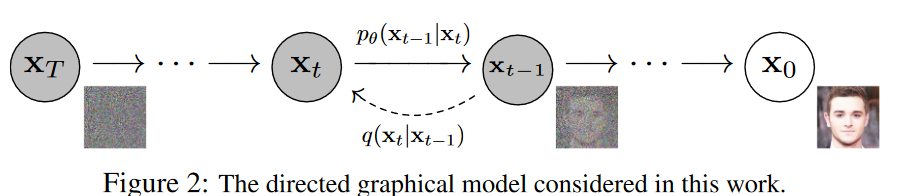
\includegraphics[width=0.8\linewidth]{figures/ddpm_fig2.png}
  \end{figure}
  \begin{itemize}
    \item Forword Process:
    \begin{figure}[!h]
      \centering
      
\includegraphics[width=1.0\linewidth]{figures/ddpm_formulation2.png}
    \end{figure}
    \item Reverse Process:
    \begin{figure}[!h]
      \centering
      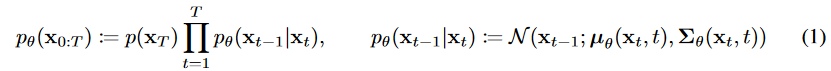
\includegraphics[width=1.0\linewidth]{figures/ddpm_formulation1.png}
    \end{figure}
  \end{itemize}
\end{frame}

\begin{frame}{Denoising Diffusion Probabilistic Models}
  % \begin{figure}[!h]
  %     \centering
  %     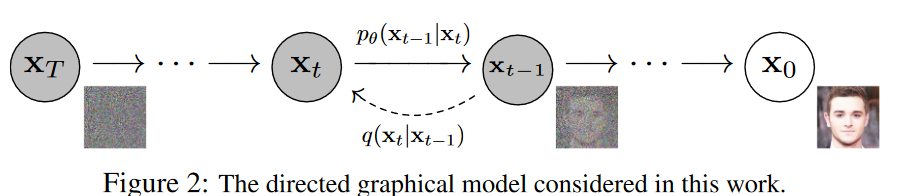
\includegraphics[width=0.8\linewidth]{figures/ddpm_fig2.png}
  % \end{figure}
  \begin{itemize}
    \item Forword Process:
    \begin{figure}[!h]
      \centering
      
\includegraphics[width=1.0\linewidth]{figures/ddpm_formulation2.png}
    \end{figure}
    \item Reparameterization trick: $ {\alpha}_t := 1-{\beta}_t, \overline{\alpha}_t := \prod \limits_{s=1}^t {\alpha}_s$
    \begin{figure}[!h]
      \centering
      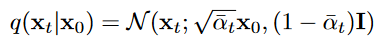
\includegraphics[width=0.5\linewidth]{figures/ddpm_formulation4.png}
    \end{figure}
    \item Objective: $E[-log p_{\theta}(x_0)]$
    % \item Reverse Process:
    \begin{figure}[!h]
      \centering
      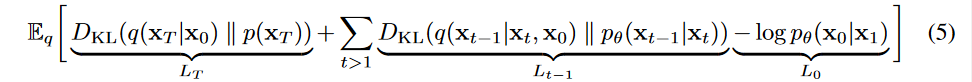
\includegraphics[width=1.0\linewidth]{figures/ddpm_formulation5.png}
      \vspace{8mm}
      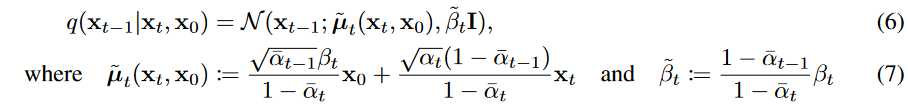
\includegraphics[width=1.0\linewidth]{figures/ddpm_formulation67.png}
    \end{figure}
  \end{itemize}
\end{frame}
\begin{frame}{Denoising Diffusion Probabilistic Models}
  DDPM Implement:
  \begin{itemize}
    \item Set ${\beta}_t$ to constants.
    \item Set $\sum_{\theta} (x_t,t)$ to constants.
    \item Objective:
    \begin{figure}[!h]
      \centering
      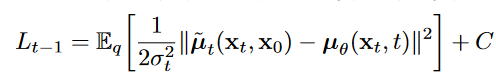
\includegraphics[width=0.7\linewidth]{figures/ddpm_formulation8.png}
    \end{figure}
    % \item Reverse Process:
    \item To minimize $L_{t-1}$:
    \begin{figure}[!h]
      \centering
      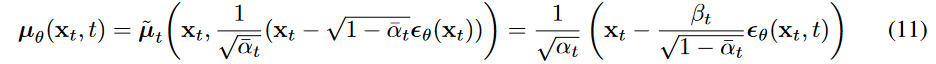
\includegraphics[width=1.0\linewidth]{figures/ddpm_formulation11.png}
    \end{figure}
    \begin{figure}[!h]
      \centering
      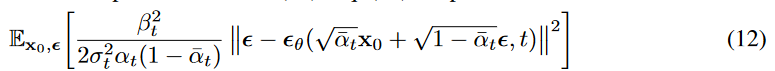
\includegraphics[width=1.0\linewidth]{figures/ddpm_formulation12.png}
    \end{figure}
  \end{itemize}
\end{frame}

\begin{frame}{Denoising Diffusion Probabilistic Models}
  DDPM Implement:
  \begin{figure}[!h]
    \centering
    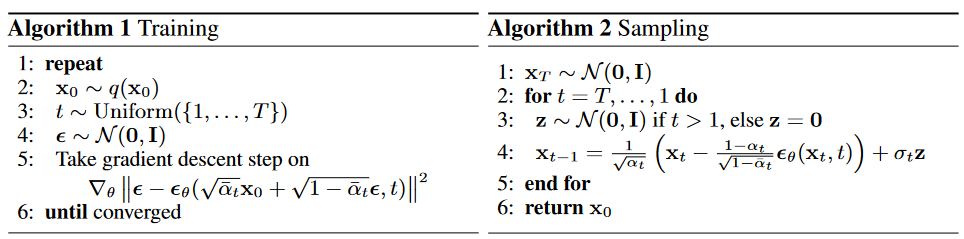
\includegraphics[width=1.0\linewidth]{figures/ddpm_algorithm.png}
  \end{figure}
\end{frame}

\section{PROTDIFF and SMCDIFF}
\begin{frame}
    \frametitle{Table of Contents}
    \tableofcontents[currentsection]
\end{frame}

\begin{frame}{PROTDIFF and SMCDIFF}
  \vspace{-3mm}
  \begin{figure}[!h]
      \centering
      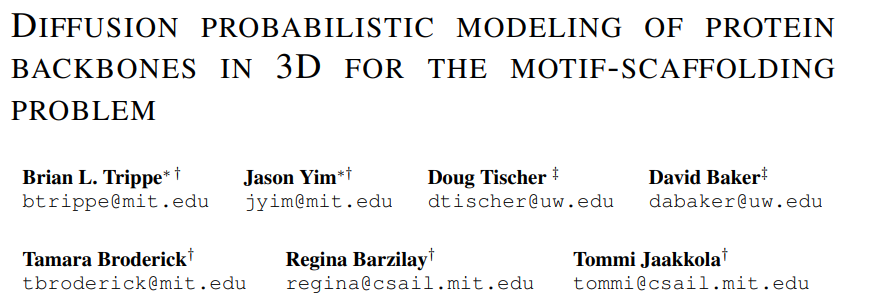
\includegraphics[width=0.9\linewidth]{figures/ProtDIFF.png}
      % 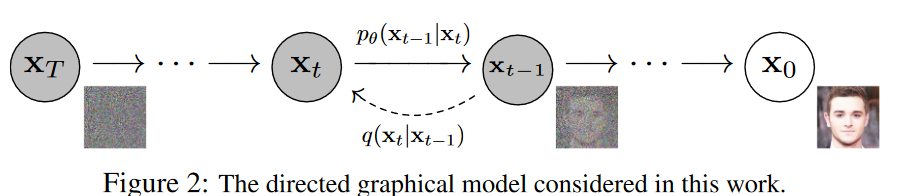
\includegraphics[width=0.8\linewidth]{figures/ddpm_fig2.png}
  \end{figure}
  \begin{itemize}
    \item Many methods do not build scaffolds longer than about 20 residues.
    \item they require hours of computation to generate a single plausible scaffold.
  \end{itemize}
\end{frame}

\begin{frame}{PROTDIFF and SMCDIFF}
  \textbf{PROTDIFF}
  \begin{itemize}
    \item Model Protein Structure: predict C-alpha only.
    \begin{itemize}
      \item E(3) euqivariant graph neural network.
      \item We associate each node with coordinates $x_n \in R^3$ and D features $h_n \in R^D$.
    \end{itemize}
    \item Trained on filtered PDB.
    \begin{itemize}
      \item protein length in range in [40, 128] and  filtered out pdb with > 5A atomic resolution, totally 4269 training samples.
    \end{itemize}
  \end{itemize}
  \textbf{SMCDIFF}
  \begin{itemize}
    \item A strategy that training unconditionally but sampling conditionally.
    \item Previous strategy have a problem:
    \begin{itemize}
      \item Forward diffuse the conditioning variable to obtain $X_M^{1:T}$ from $q(X_M^{1:T}|X_M^{(0)})$
      \item For each t, sample $X_S^{t}$ from $p_{\theta}(X_S^{t}|X_M^{(t+1)}, X_S^{(t+1)})$
    \end{itemize}
    % \begin{figure}[!h]
    %   \centering
    %   % 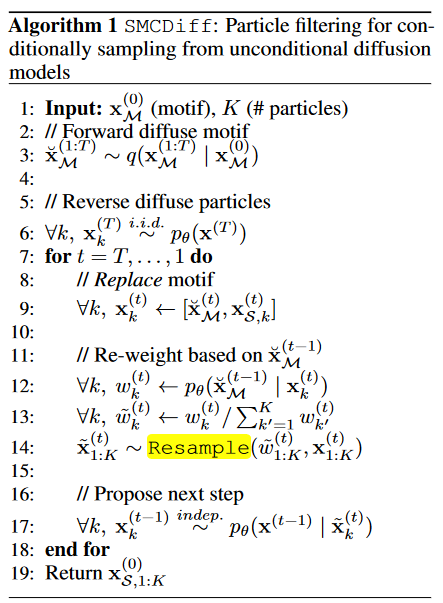
\includegraphics[width=0.4\linewidth]{figures/ProtDIFF_algorithm.png}
    %   % 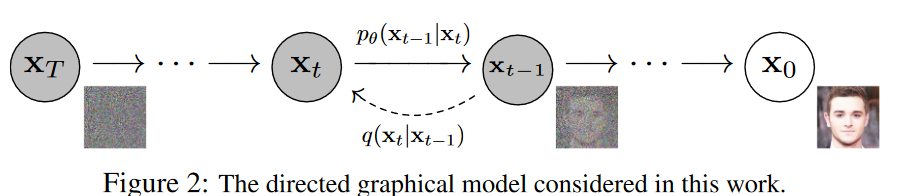
\includegraphics[width=0.8\linewidth]{figures/ddpm_fig2.png}
    % \end{figure}
  \end{itemize}
\end{frame}

\begin{frame}{PROTDIFF and SMCDIFF}
  \textbf{SMCDIFF}
  \begin{itemize}
    \item A strategy that training unconditionally but sampling conditionally.
    % \begin{figure}[!h]
    %   \centering
    %   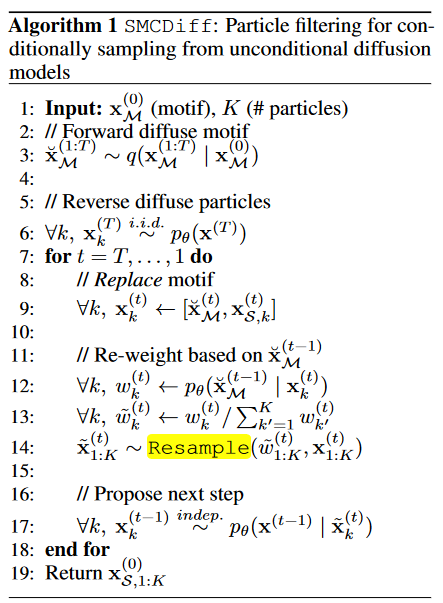
\includegraphics[width=0.4\linewidth]{figures/ProtDIFF_algorithm.png}
    % \end{figure}

    \begin{figure}
      \centering
      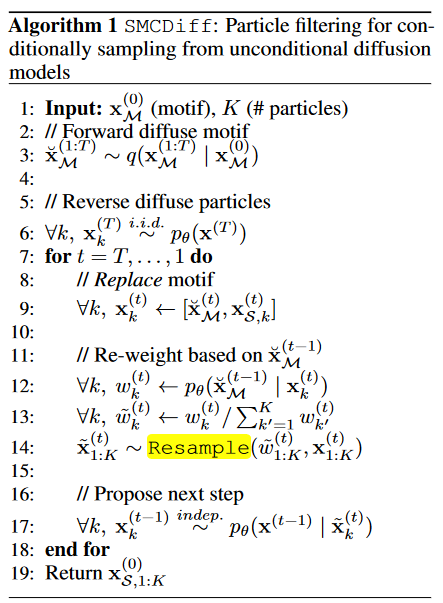
\includegraphics[width=0.4\linewidth]{figures/ProtDIFF_algorithm.png}
      % \hspace{1in}
      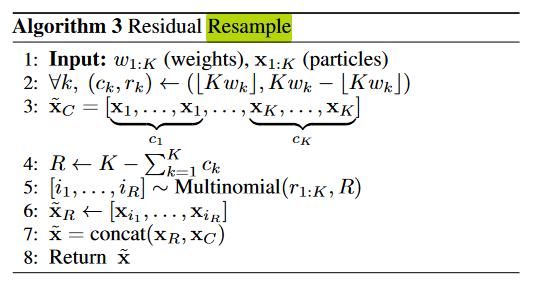
\includegraphics[width=0.5\linewidth]{figures/ProtDIFF_algorithm_resample.png}
      % \caption{两张图片并排在一个浮动体}
    \end{figure}
  \end{itemize}
\end{frame}

\begin{frame}{PROTDIFF and SMCDIFF}
  \textbf{Experiments: conditional}\\
  Evaluation: For a given backbone, firstly generate protein sequence by ProteinMPNN, then predict its backbone by Alphafold2. Compare the given backbone and the AF2-version backbone (by RMSD or TM score).
  \begin{itemize}
    \item Ablation on SMCDIFF. 
    \begin{figure}[!h]
      \centering
      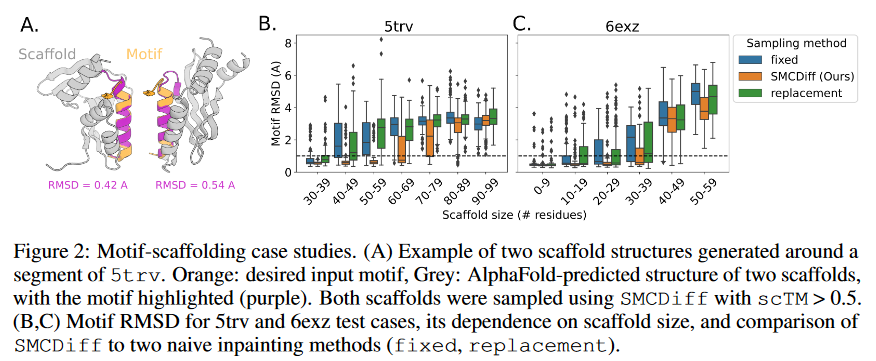
\includegraphics[width=0.9\linewidth]{figures/ProtDIFF_fig2.png}
      % 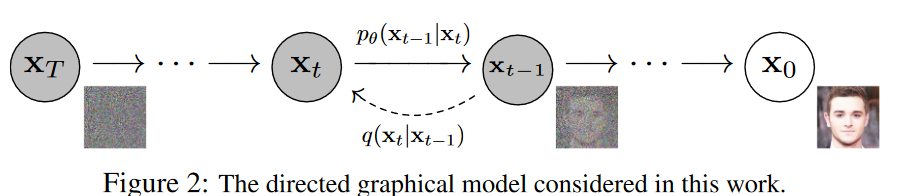
\includegraphics[width=0.8\linewidth]{figures/ddpm_fig2.png}
  \end{figure}
  \end{itemize}
\end{frame}

\begin{frame}{PROTDIFF and SMCDIFF}
  \textbf{Experiments: unconditional}\\
  Evaluation: For a given backbone, firstly generate protein sequence by ProteinMPNN, then predict its backbone by Alphafold2. Compare the given backbone and the AF2-version backbone (by RMSD or TM score).
  % \begin{itemize}
    % \item Ablation on SMCDIFF. 
  \begin{figure}[!h]
    \centering
    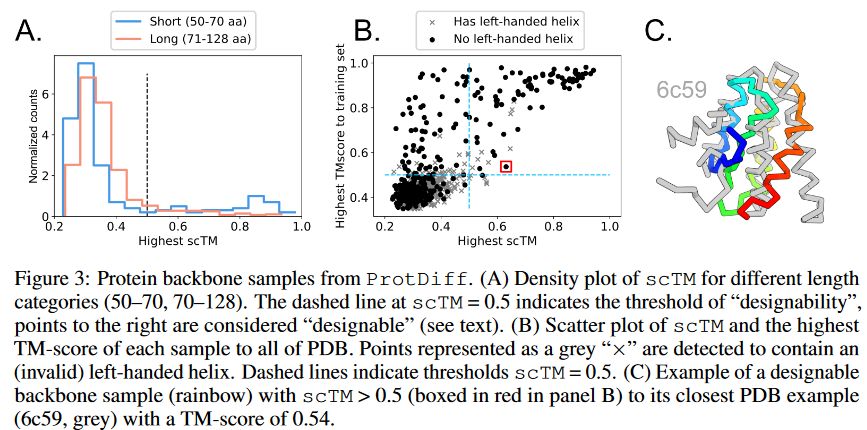
\includegraphics[width=0.9\linewidth]{figures/ProtDIFF_fig3.png}
    % 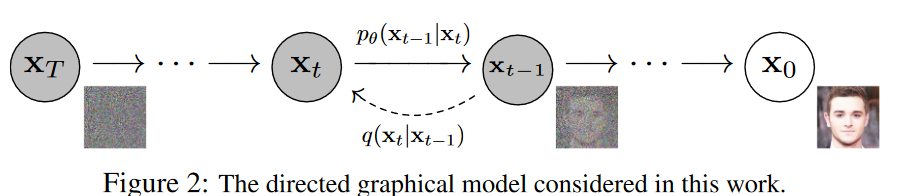
\includegraphics[width=0.8\linewidth]{figures/ddpm_fig2.png}
  \end{figure}
  % \end{itemize}
\end{frame}


\section{FoldingDiff}
\begin{frame}
    \frametitle{Table of Contents}
    \tableofcontents[currentsection]
\end{frame}

\begin{frame}{FoldingDiff}
  \vspace{-3mm}
  \begin{figure}[!h]
      \centering
      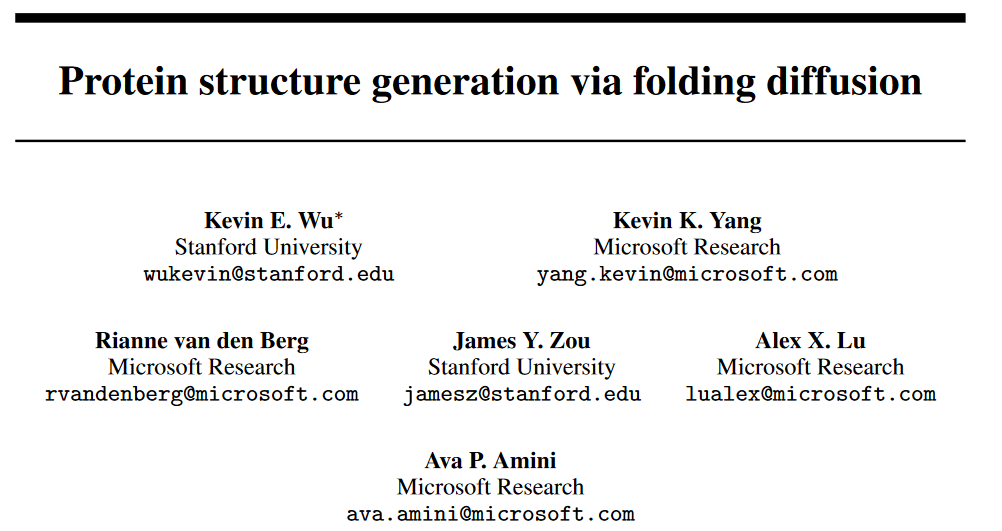
\includegraphics[width=0.9\linewidth]{figures/Foldingdiff.png}
  \end{figure}
  \vspace{-3mm}
  \begin{itemize}
    \item Previous rely on complex equivariant network architectures or loss functions to learn to generate a 3D point cloud.
    \item We introduce a model that acts on the inter-residue angles in protein backbones instead of on Cartesian atom coordinates.
  \end{itemize}
\end{frame}

\begin{frame}{FoldingDiff}
  \textbf{Method}
  \vspace{-3mm}
  \begin{figure}[!h]
      \centering
      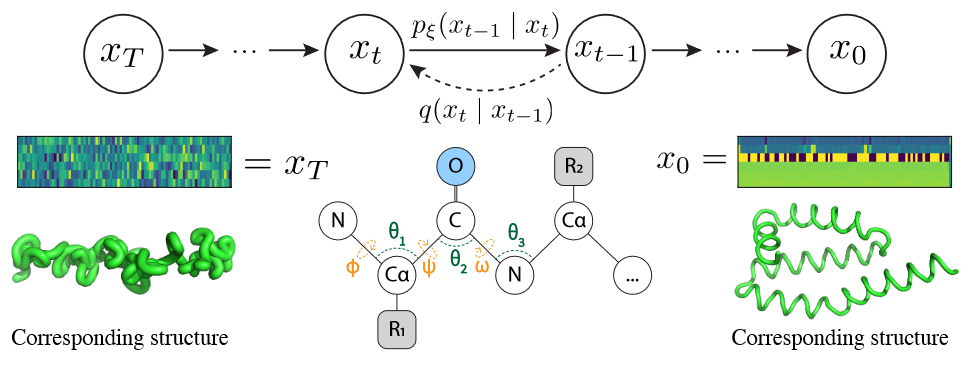
\includegraphics[width=0.9\linewidth]{figures/Foldingdiff_fig1.png}
  \end{figure}
  \vspace{-3mm}
  \begin{itemize}
    \item model: Transformer.
    \item Trained on CATH.
  \end{itemize}
\end{frame}

\begin{frame}{FoldingDiff}
  \textbf{Method}
  \begin{itemize}
    \item Add noise and denoise (Using wrapped normal).
    \begin{figure}[!h]
      \centering
      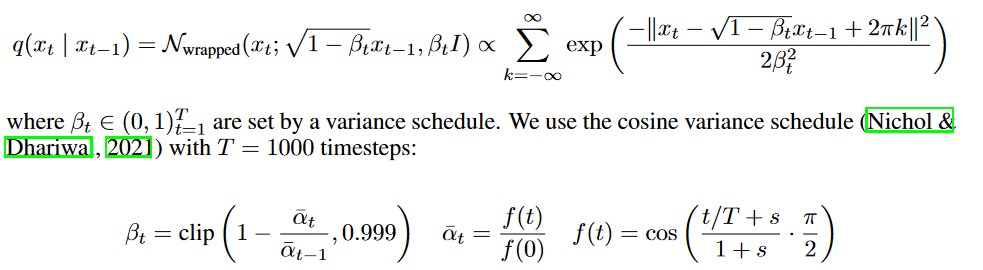
\includegraphics[width=0.9\linewidth]{figures/Foldingdiff_formulation.png}
    \end{figure}
    \item Loss.
    \begin{figure}[!h]
      \centering
      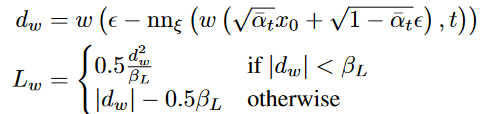
\includegraphics[width=0.6\linewidth]{figures/Folding_loss.png}
    \end{figure}
  \end{itemize}
  \vspace{-3mm}
  \begin{figure}[!h]
      \centering
      % 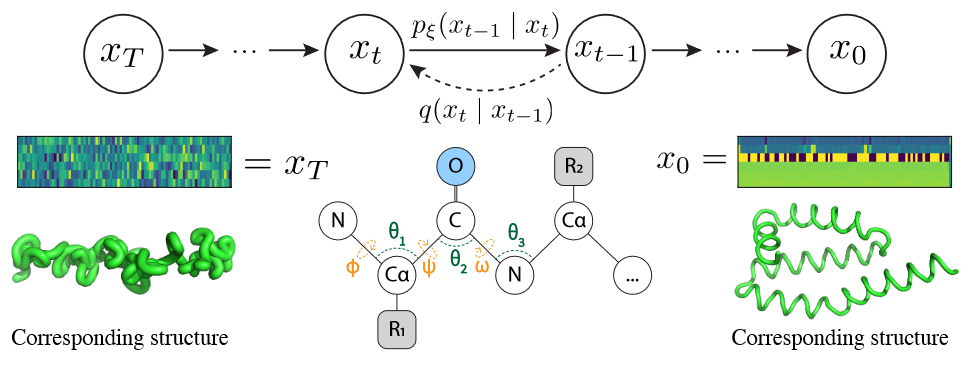
\includegraphics[width=0.9\linewidth]{figures/Foldingdiff_fig1.png}
  \end{figure}
  \vspace{-3mm}
\end{frame}

\begin{frame}{FoldingDiff}
  \textbf{Method}
  \begin{figure}[!h]
    \centering
    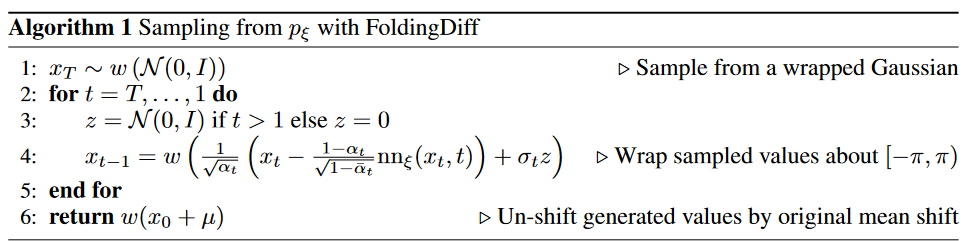
\includegraphics[width=1.0\linewidth]{figures/Foldingdiff_algorithm.png}
  \end{figure}
\end{frame}

\begin{frame}{FoldingDiff}
  \textbf{Experiments}
  \begin{figure}[!h]
    \centering
    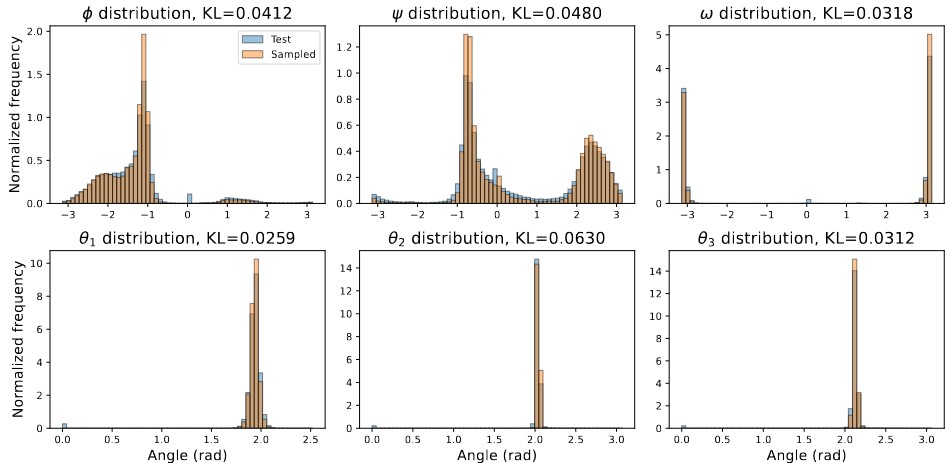
\includegraphics[width=1.0\linewidth]{figures/Foldingdiff_fig2.png}
  \end{figure}
\end{frame}

\begin{frame}{FoldingDiff}
  \textbf{Experiments}
  \begin{figure}[!h]
    \centering
    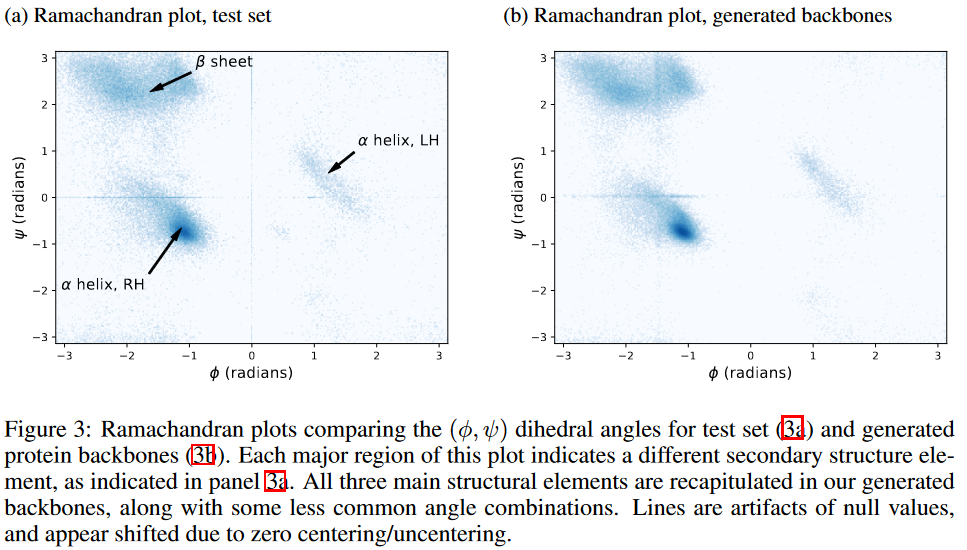
\includegraphics[width=1.0\linewidth]{figures/Foldingdiff_fig3.png}
  \end{figure}
\end{frame}

\begin{frame}{FoldingDiff}
  \textbf{Experiments}
  \begin{figure}[!h]
    \centering
    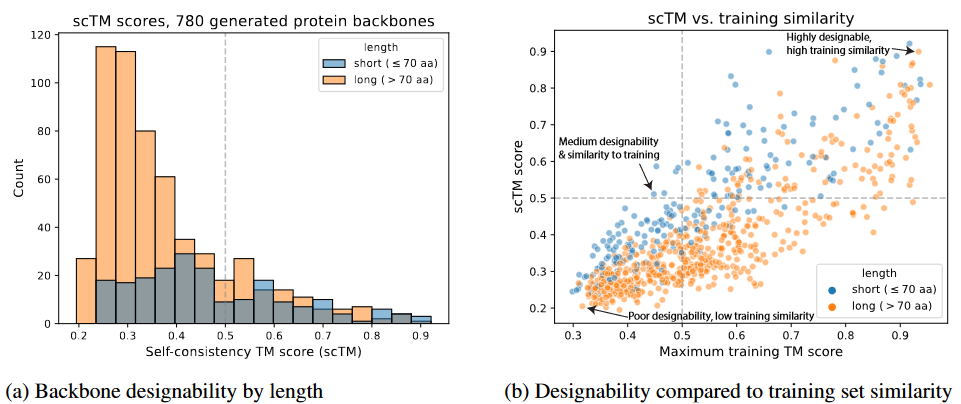
\includegraphics[width=1.0\linewidth]{figures/Foldingdiff_fig5.png}
  \end{figure}
\end{frame}

\begin{frame}{FoldingDiff}
  Reject.
  \begin{itemize}
    \item Metrics.
    \item Baselines.
  \end{itemize}
\end{frame}

\end{document}